\documentclass{article}

%\usepackage{corl_2023} % Use this for the initial submission.
\usepackage[final]{corl_2023} % Uncomment for the camera-ready ``final'' version.
%\usepackage[preprint]{corl_2023} % Uncomment for pre-prints (e.g., arxiv); This is like ``final'', but will remove the CORL footnote.

\usepackage{graphicx}
\usepackage{amssymb}
\usepackage{amsmath}
\usepackage{listings}
\usepackage{subcaption}
\usepackage{latexsym}
\usepackage{amsthm}
\usepackage{natbib}
\usepackage{listings}
\usepackage{hyperref} 

\title{Exercise 2 - Robot Learning Course}

% The \author macro works with any number of authors. There are two
% commands used to separate the names and addresses of multiple
% authors: \And and \AND.
%
% Using \And between authors leaves it to LaTeX to determine where to
% break the lines. Using \AND forces a line break at that point. So,
% if LaTeX puts 3 of 4 authors names on the first line, and the last
% on the second line, try using \AND instead of \And before the third
% author name.

% NOTE: authors will be visible only in the camera-ready and preprint versions (i.e., when using the option 'final' or 'preprint'). 
% 	For the initial submission the authors will be anonymized.

\author{
  Andrea Ongaro\\
	Computer Engineering\\
	Politecnico di Torino, Italy\\
	\texttt{s329706@studenti.polito.it} \\
  %% examples of more authors
  %% \And
  %% Coauthor \\
  %% Affiliation \\
  %% Address \\
  %% \texttt{email} \\
  %% \AND
  %% Coauthor \\
  %% Affiliation \\
  %% Address \\
  %% \texttt{email} \\
  %% \And
  %% Coauthor \\
  %% Affiliation \\
  %% Address \\
  %% \texttt{email} \\
  %% \And
  %% Coauthor \\
  %% Affiliation \\
  %% Address \\
  %% \texttt{email} \\
}


\begin{document}
\maketitle

%===============================================================================

\begin{abstract}
This article is part of a series of three articles for the Reinforcement Learning course in Politecnico di torino. 
In this article, the second one, we analyze the potentiality of the q-learning in the context of open AI gym, specifically in the Cart Pole changing different value of epsilon and different initialization of the q-table. 

\end{abstract}

% Two or three meaningful keywords should be added here
\keywords{Reinforcement Learning, Robots, AI} 

%===============================================================================

\section{Introduction}
\subsection{The system - CartPole-v0}
CartPole-v0 system from OpenAI is part of the classic control environment and it's been used the sample code provided by \href{https://www.polito.it/personale?p=andrea.protopapa}{Andrea Protopapa} in the course of Reinforcement Learning. Information about this system is sourced from the official documentation \cite{Cart_pole} and its GitHub repository. Below is the definition provided by the authors for CartPole-v0\\ \\
\textit{This environment corresponds to the version of the cart-pole problem described by Barto, Sutton, and Anderson in “Neuronlike Adaptive Elements That Can Solve Difficult Learning Control Problem”. A pole is attached by an un-actuated joint to a cart, which moves along a frictionless track. The pendulum is placed upright on the cart and the goal is to balance the pole by applying forces in the left and right direction on the cart.\citep{Cart_pole}}

\begin{figure}[h]
	\centering
	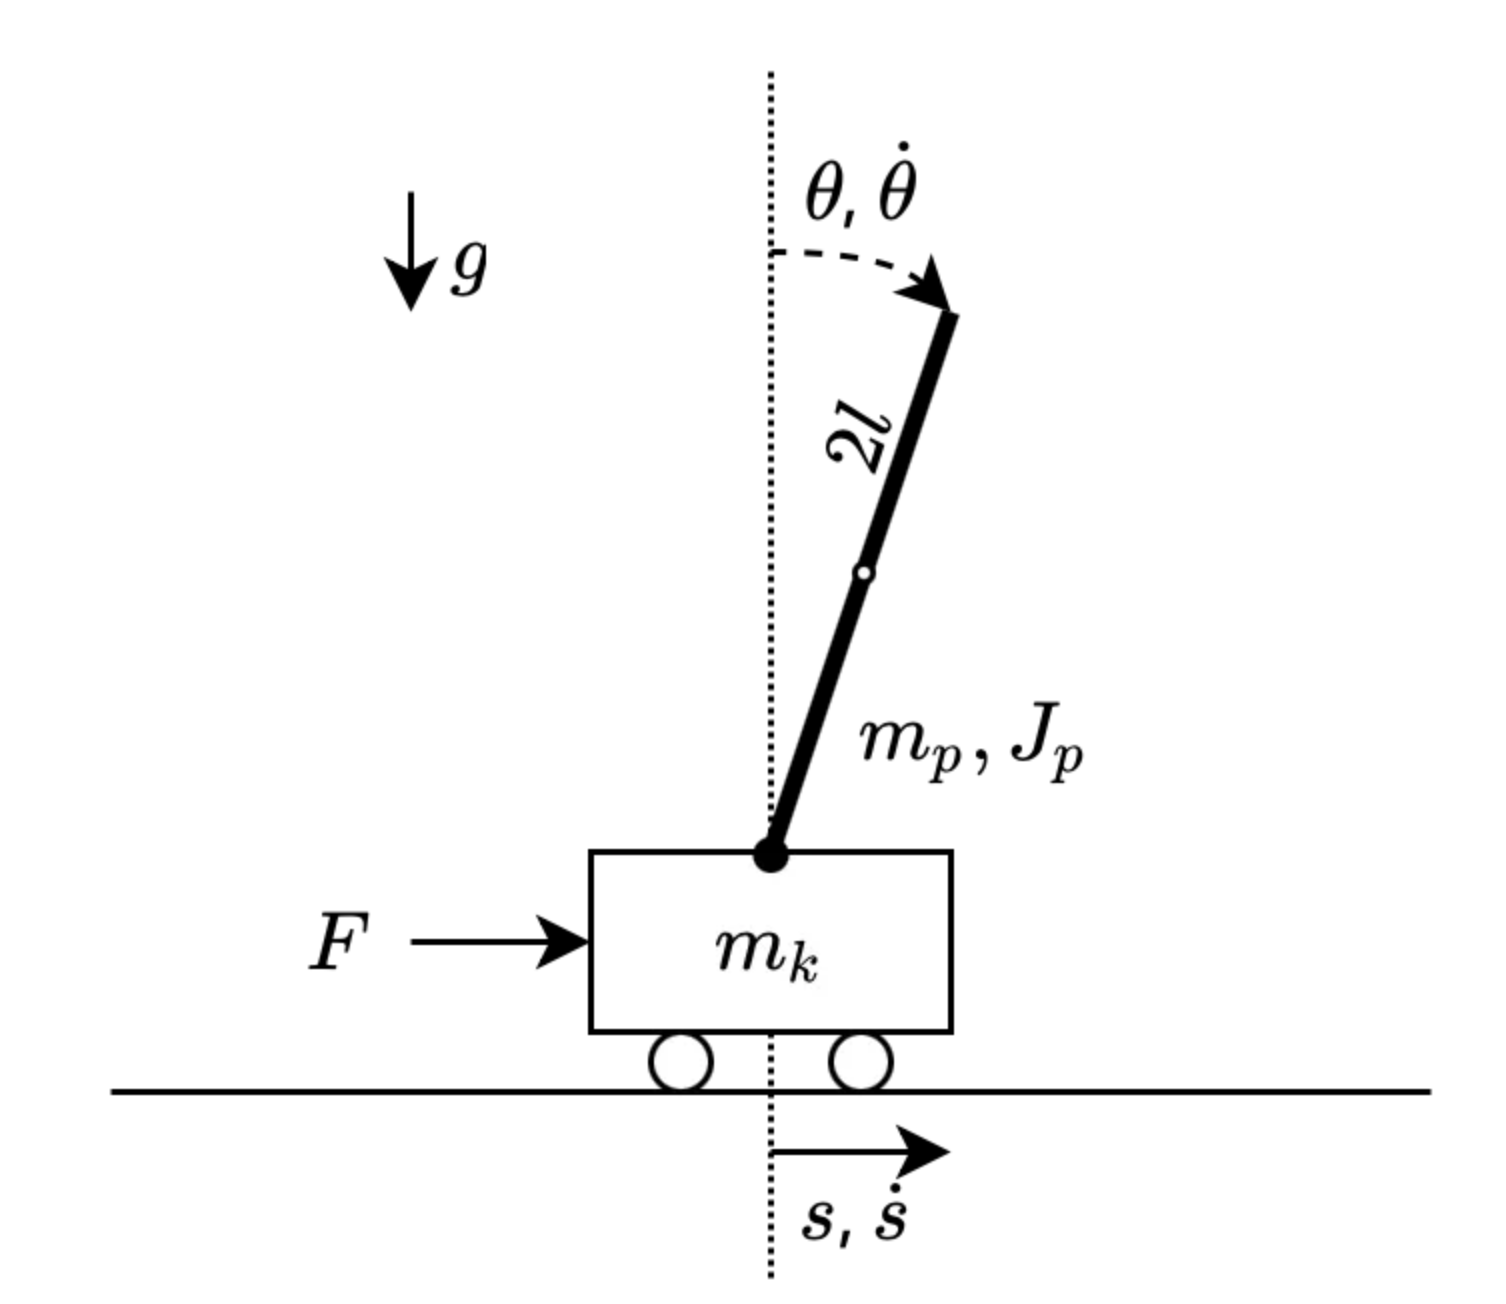
\includegraphics[width=0.5\linewidth]{../data/images/cart.png}
	\caption{Graphical explation about the whole system}
	\label{fig:plot1}
\end{figure}
The observation is a four element vector: 
\begin{figure}[h]
	\centering
	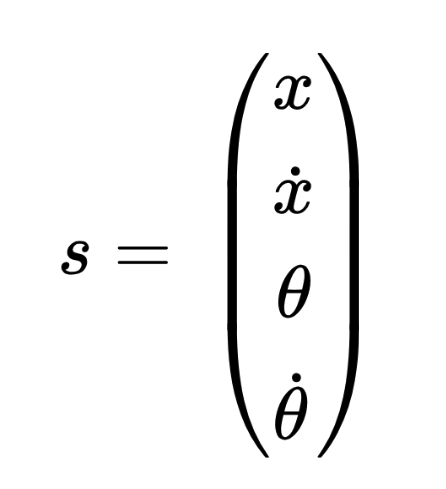
\includegraphics[width=0.2\linewidth]{../data/images/vector.png}
	\caption{Observation vector}
	\label{fig:plot1}
\end{figure}

where 
\begin{itemize}
	\item $x$: the position of the cart
	\item $\dot{x}$: the velocity, 
	\item $\theta$:  the angle of the pole
	\item $\dot{\theta}$: the angular velocity of the pole., 	
\end{itemize}

\subsection{Q-Learning}
Q-learning is a model-free algorithm. We can think of model-free algorithms as trial-and-error methods. The agent explores the environment and learns from outcomes of the actions directly, without constructing an internal model or a Markov Decision Process.
In the beginning, the agent knows the possible states and actions in an environment. Then the agent discovers the state transitions and rewards by exploration.

\subsubsection{Exploration vs. Exploitation Tradeoff}
The agent tries to discover its environment. During these trials, an agent has a set of actions to select from. Some of the actions are previously selected and the agent might guess the outcome. On the other hand, some actions are never taken before.\\ \\
The concept of exploiting what the agent already knows versus exploring a random action is called the exploration-exploitation trade-off.
When the agent \textbf{explores}, it can improve its current knowledge and gain better rewards in the long run. However, when it \textbf{exploits}, it gets more reward immediately, even if it is a sub-optimal behavior.  \\ \\
As the agent can’t do both at the same time, there is a trade-off. Initially the agent doesn’t know the outcomes of possible actions. Hence, sufficient initial exploration is required. If some actions lead to better rewards than others, we want the agent to select these options. However, only exploiting what the agent already knows is a dangerous approach.

\subsubsection{$\epsilon$ greedy}
In Q-learning, we select an action based on its reward. The agent always chooses the optimal action. Hence, it generates the maximum reward possible for the given state.\\
In epsilon-greedy policy, the agent uses both exploitations to take advantage of prior knowledge and exploration to look for new options \ref{fig:expl}.

The epsilon-greedy approach selects the action with the highest estimated reward most of the time. The aim is to have a balance between exploration and exploitation. Exploration allows us to have some room for trying new things, sometimes contradicting what we have already learned.  

With a small probability of $\epsilon$, we choose to explore, i.e., not to exploit what we have learned so far. In this case, the action is selected randomly, independent of the action-value estimates.
As we’ve discussed above, usually the optimal action, i.e., the action with the highest Q-value is selected. Otherwise, the algorithm explores a random action.

\begin{figure}[h]
	\centering
	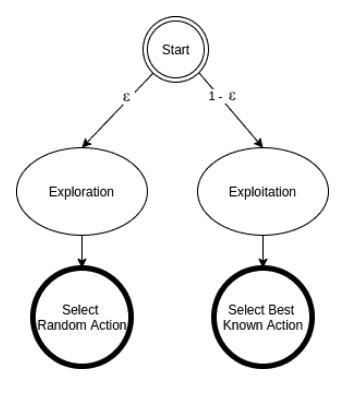
\includegraphics[width=0.5\linewidth]{../data/images/exp_e.png}
	\caption{Exploitation vs Exploration \cite{q_le}}
	\label{fig:expl}
\end{figure}

\subsubsection{Heatmap}
To analyze the current state of the analyzed system it's possible to used an heatmap. The heatmap depicts values for a main variable of interest across two axis variables as a grid of colored squares. The axis variables are divided into ranges like a bar chart or histogram, and each cell’s color indicates the value of the main variable in the corresponding cell range \cite{heatmap}. \\ 

High-Value Regions:
•	Represent states where the agent expects to receive high cumulative rewards.
•	For example, in the cart-pole problem:
•	States near the upright position (balanced pole) with low velocity and angular velocity likely have higher values.

Low-Value Regions:
•	Represent states leading to termination or failure (e.g., the pole falling or the cart moving out of bounds).
•	For the cart-pole, states with extreme angles or high velocities might have low values.

 

\subsubsection{GLIE - greedy in limit with infinite exploration}
-	Each action is executed infinitely often in every state that is visited infinitely often;
-	In the limit, the learning policy is greedy with respect to the Q-value function with probability 1

\section{Process - Another name}
\subsection{Epsilon value}
During this expirement we developed three different stategies that we are going to compare, in this subsection we are going to compare the first two. The first one with a costant epsilon  ($\epsilon =  0.2$) while the second with the following formula \ref{formula:epsilon} such that epsilon reaches 0.1 after k=20000 episodes (round b to nearest integer). In order to do this we have set the value of b as 2221 and in the end of the glie schedule we'll have epsilon exactly equal to $0.09995049727735025$

\centering
\label{formula:epsilon}
$ e_k = b / (b+k) $ 

\flushleft

\subsubsection{Fixed $\epsilon$ vs GLIE epsilon schedule}
Speaking about the performance between a fixed epsilon vs. the GLIE epsilon schedule 

Plot the return obtained at each training episode, to view how the training process has
progressed

Looking at the testing render you can see an improvement compared to the fixed epsilon so there is an higher change see the pole mantain the stability, but it's not perfect anyway.

\begin{figure}[h]
	\centering
	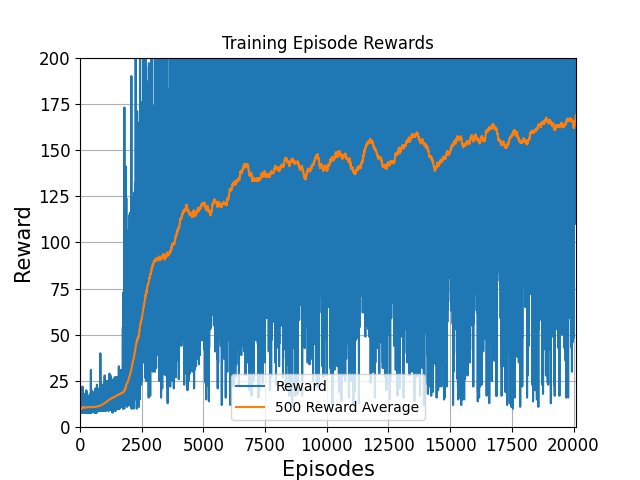
\includegraphics[width=0.5\linewidth]{../data/plot/q_learning_constant_0.2.png}
	\caption{Return obtained at each training episode - $\epsilon = 2$}
	\label{fig:costant_eps}
\end{figure}

\begin{figure}[h]
	\centering
	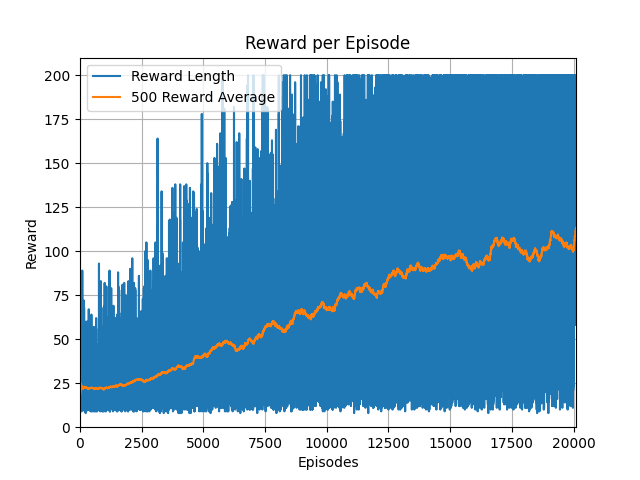
\includegraphics[width=0.5\linewidth]{../data/plot/q_learning_GLIE.png}
	\caption{Return obtained at each training episode - $\epsilon$ get from the formula \ref{formula:epsilon}}
	\label{fig:glie_eps}
\end{figure}

\subsection{Value function}
After computing the associated value function  $d$ we generate the heatmap of the computed value function in terms of $ x $ and $\dot{\theta}$, (the current position of the cart and the pole angle) and therefore average the values
over $\dot{x} $ and $\dot{\theta} $ for plotting.


\begin{figure}[h]
	\centering
	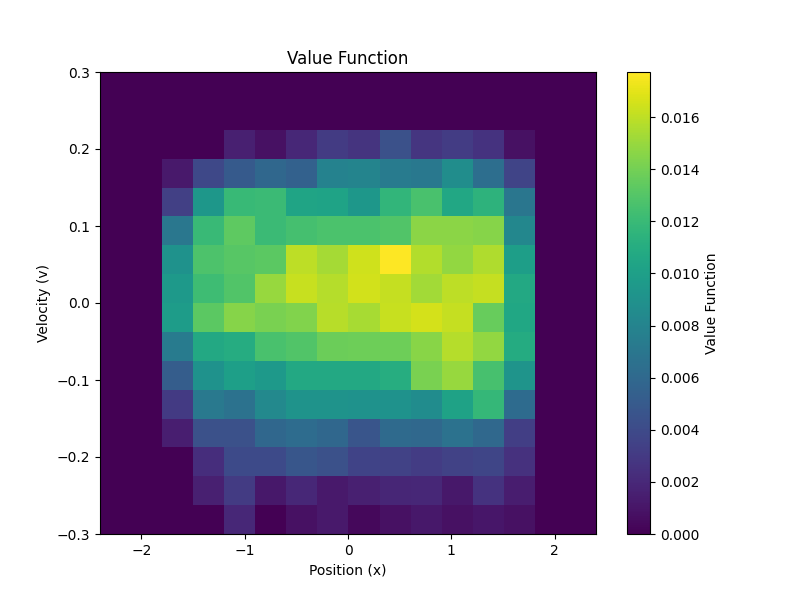
\includegraphics[width=0.5\linewidth]{../data/plot/heatmap_full_training_constant_0.2.png}
	\caption{Heatmap image for q-learning with costant epsilon}
	\label{fig:plot1}
\end{figure}
\begin{figure}[h]
	\centering
	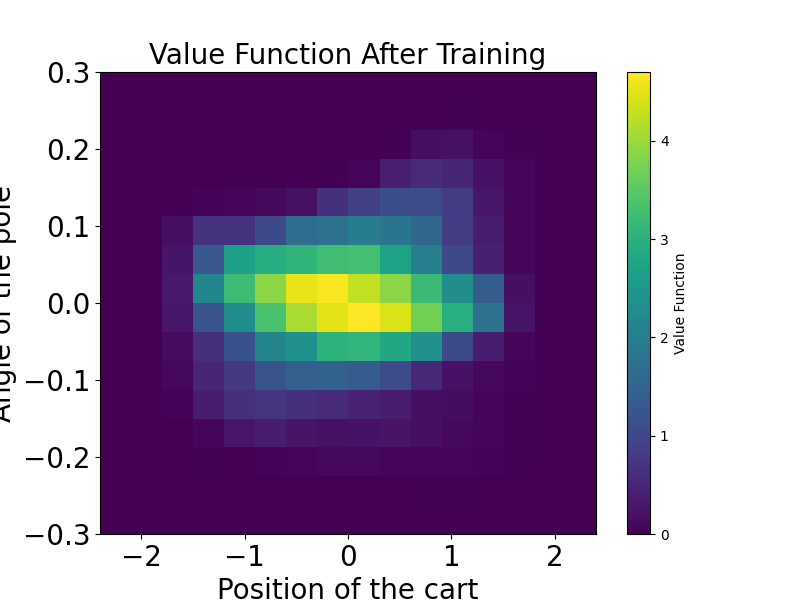
\includegraphics[width=0.5\linewidth]{../data/plot/heatmap_full_training_GLIE.png}
	\caption{Heatmap image for q-learning with glie epsilon schedule}
	\label{fig:plot1}
\end{figure}

After the full training The agent has effectively learned the optimal policy and accurately estimates V(s) and the heatmap is clear and smooth, with distinct high-value regions corresponding to optimal states or policies.

Now, we can take into consideration other states in which you can analyze the system.

\pagebreak

\subsubsection{Before training}
Before training the heatmap is likely flat, with no clear structure. All state-action pairs have equal zero Q -values, meaning  the value function is uniform across states. The agent has no prior knowledge of the environment.

\begin{figure}[h]
	\centering
	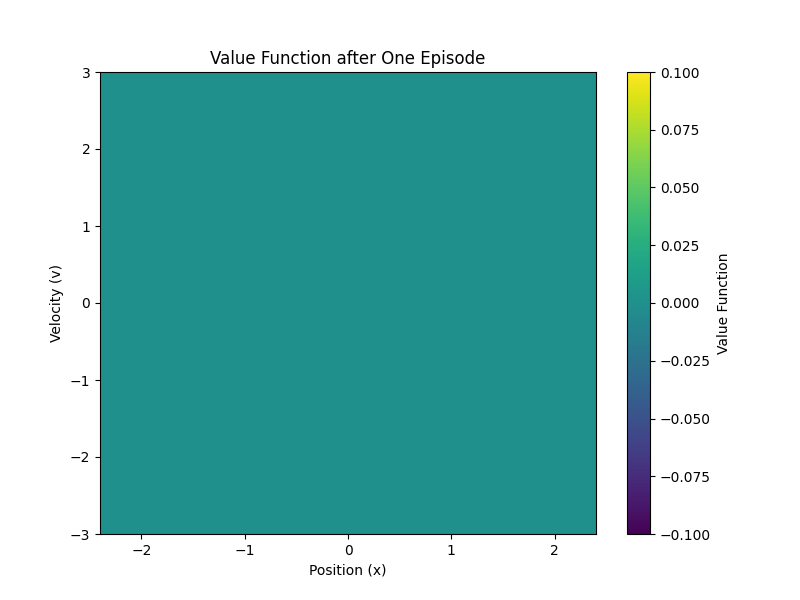
\includegraphics[width=0.5\linewidth]{../data/plot/heatmap_initial_training_constant_0.2.png}
	\caption{Heatmap in the initial state}
	\label{fig:plot1}
\end{figure}

\subsubsection{After one episode}
Some regions of the heatmap may start showing slightly higher values, particularly in states visited during the episode.
•	The updates are sparse and localized around the trajectory the agent followed during the episode.
•	Unvisited states still retain their initial values. the agent updates the Q-values for the specific states and actions it encountered, improving its estimate of  V(s)  in those regions.
•	Most of the state space remains unexplored, leading to minimal structure in the heatmap.
\begin{figure}[h]
	\centering
	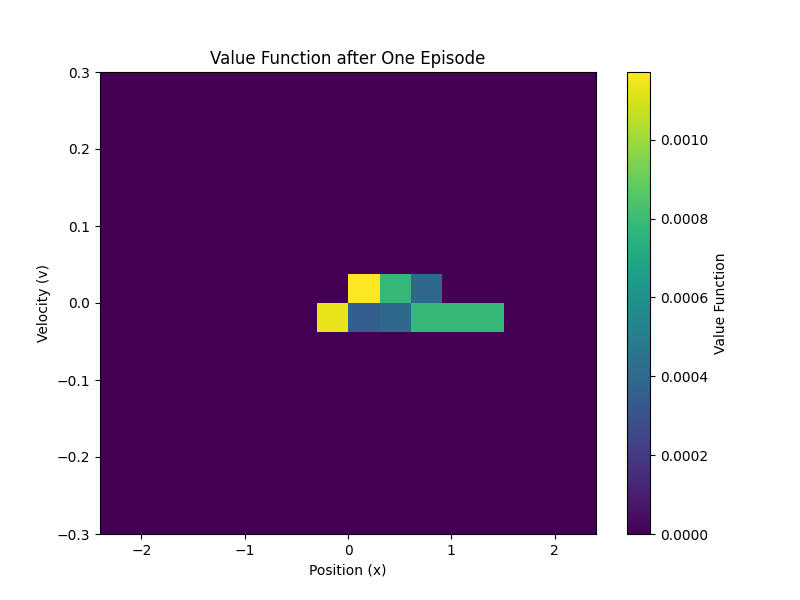
\includegraphics[width=0.5\linewidth]{../data/plot/heatmap_after_one_episode_constant_0.2.png}
	\caption{Heatmap in the initial state}
	\label{fig:plot1}
\end{figure}

\subsubsection{Half-way training}
The heatmap begins to take shape, showing a clearer distinction between “good” and “bad” states.
•	High-value regions correspond to states closer to the goal or those leading to higher rewards.
•	Low-value regions reflect states where the agent expects poor outcomes or failures.
•	Some areas might still be noisy or less structured, especially in underexplored regions.
\begin{figure}[h]
	\centering
	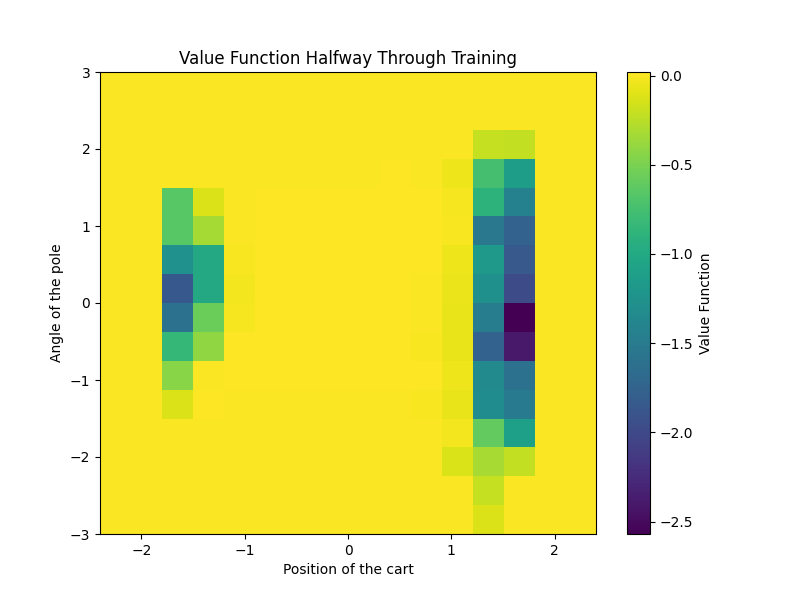
\includegraphics[width=0.5\linewidth]{../data/plot/heatmap_halfway_constant_0.2.png}
	\caption{Halfway Training Heatmap}
	\label{fig:plot1}
\end{figure}


\subsection{Epsilon zero}
What's the meaning in setting epsilon zero? There is not exploration stage, it will always use an known action. No reason to do this
In this subsection we experiment epsilon equal to zero in two different casisticts:
\begin{itemize}
	\item keeping the initial Q-function values at zero;
	\item setting the initial Q-function values at 50 for all states and actions;
\end{itemize}

- In which case does the model perform better?
- Why is this the case? How does the initialization of Q values affect exploration?

\section{Q-Learning : Different applications}

\subsection{Continuous state spaces}
Q-learning can be adapted for environments with continuous state spaces, but it requires some modifications because the algorithm inherently relies on a discrete state-action table. A common approaches for continuous State spaces
is to use a state discretization, as it's been done in this article.
•	Divide the continuous state space into discrete bins (grids).
•	Each bin represents a discrete state, and standard Q-learning operates on this discretized state space.
There is an important thing to notice that discretization can lead to loss of precision and suffers from the “curse of dimensionality”\cite{article} in high-dimensional spaces.
To overcome this problem there is an alternative that involves the use of the function approximators (e.g., neural networks, decision trees, or linear regression) to represent the Q-function Q(s, a) instead of a table. This permits to handles continuous state spaces directly without discretization and scales better to high dimensions. This is the foundation of Deep Q-Learning (DQN), where neural networks approximate Q(s, a).

\subsection{Continuous action spaces}
Risposta da dare studiando molto di più.

%===============================================================================

%===============================================================================

\section{Conclusion}

Domande: 
perchè faccio l'average sugli altri due dati. Non capisco.
E' giusto che comunque faccia schifo i primi due, quello costante e quello con la formula. Con la formula migliora, ma non così tanto. Vuol dire che non sta trovando la policy ottimale?

Quale heatmap devo analizzare? E' uguale tanto il pattern dovrebbe essere sempre quello indipendente dall'epsilon impostato. Prima poi, poi sempre un po' di più.

Standard deviation è molto alta sempre mi sa.

\label{sec:conclusion}

%===============================================================================

% no \bibliographystyle is required, since the corl style is automatically used.
\bibliography{example}  % .bib

\end{document}
